\chapter{Results and analysis}
\label{sec:results}

\section{Vocabulary coverage}
\paragraph{English.} Two words in three that a reader of the English Qur'an and hadith meets already have an ASL sign
(Table~\ref{tab:coverage}). The gap is concentrated: the 50 most frequent uncovered words would raise occurrence coverage
to 77.1\%, the top 100 to 79.6\%, the top 200 to 82.7\% and the top 500 to 87.6\% (Figure~\ref{fig:covcurve}). The most
frequent uncovered words are \emph{upon} and \emph{blessings}, nearly all from the formula ``peace and blessings be upon
him'' (\ar{ﷺ}), which a single sign can render; then \emph{indeed, whoever, among, almighty, companions, deeds,
punishment, reward, mercy, believers, worship, knowledge, judgment, disbelievers, hereafter, wealth, refuge, righteous,
forgiveness, faith}.

\begin{table}[ht]
\centering\small
\caption{ASL lexicon (3,055 glosses) coverage of the English Qur'an and hadith corpora.}
\label{tab:coverage}
\begin{tabular}{l l r r r r}
\toprule
Corpus & Words counted & Distinct & Distinct covered & Occurrences & Occurrences covered \\
\midrule
Qur'an & vocabulary (no names) & 5,085 & 1,952 (38.4\%) & 68,888 & 44,212 (64.2\%) \\
Hadith & vocabulary (no names) & 11,466 & 3,431 (29.9\%) & 322,472 & 215,971 (67.0\%) \\
Both & vocabulary (no names) & 12,387 & 3,582 (28.9\%) & 391,360 & \textbf{260,183 (66.5\%)} \\
Both & content words & 13,529 & 3,624 (26.8\%) & 425,556 & 268,782 (63.2\%) \\
Both & all words & 13,612 & 3,677 (27.0\%) & 865,157 & 527,843 (61.0\%) \\
\bottomrule
\end{tabular}
\end{table}

\paragraph{Concept coverage.} Signing is by concept, not by English word: \emph{deeds} is signed WORK, \emph{forbade}
FORBID, \emph{faith} BELIEVE, while \emph{indeed} or \emph{verily} are not signed. The LLM proposed, for 424 of the
most frequent uncovered words, an existing gloss with the same meaning, ``not signed'', or ``needs a new sign''. With
those proposals, 70.8\% of occurrences can be signed with the current lexicon (73.7\% when unsigned function words are
set aside); words that need a new sign (\emph{prostration, lawful, guidance, resurrection, revelation, repentance,
decree, patience, intention, throne}) account for 8.5\% of occurrences among the words examined. These mappings are
proposals pending review by Deaf signers and are reported separately from the direct coverage.

\begin{figure}[ht]
\centering
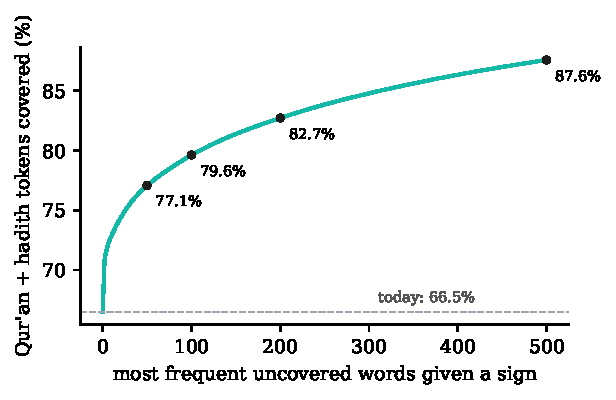
\includegraphics[width=0.62\textwidth]{figures/coverage_curve_en.pdf}
\caption{Occurrence coverage of the English Qur'an and hadith if the most frequent uncovered words were given a sign.}
\label{fig:covcurve}
\end{figure}

\begin{sloppypar}\noindent\textbf{Arabic.} The same count for the Arabic Qur'an and hadith with the ArSL lexicon (Table~\ref{tab:coverage_ar})
gives 59.6\% of all word occurrences and 53.3\% of content-word occurrences. Two
differences from English must be kept in mind. First, Arabic attaches conjunctions, prepositions and pronouns to words
(\ar{فقال}, \ar{عنه}, \ar{منها}), so the count of \emph{distinct} surface forms (62,562) is far larger than the number of
lemmas and the distinct-word figure (23.9\%) understates coverage. Second, Arabic has no capital letters, so proper names
cannot be detected the same way and remain in the count: \ar{عمر}, \ar{أبو هريرة}, \ar{عائشة}, \ar{أبو بكر}, \ar{أنس},
\ar{ابن عباس} are among the most frequent uncovered words, together with the formulas \ar{صلى الله عليه وسلم} and
\ar{عز وجل}. The real gaps are content words such as \ar{القيامة}, \ar{الدنيا}, \ar{القرآن} and \ar{شيء}, which are the
next signs to collect. Starting from the 53.3\% of content-word occurrences, the 50, 100, 200 and 500 most frequent uncovered forms would
raise coverage to 64.0\%, 66.5\%, 69.0\% and 72.9\%. (This run counted 3,948 glosses: the 31 letter signs are
excluded.)
\end{sloppypar}

\begin{table}[ht]
\centering\small
\caption{ArSL lexicon coverage of the Arabic Qur'an and hadith corpora. Distinct
counts are of surface forms with clitics.}
\label{tab:coverage_ar}
\begin{tabular}{l l r r r r}
\toprule
Corpus & Words counted & Distinct & Distinct covered & Occurrences & Occurrences covered \\
\midrule
Qur'an & content words & 14,603 & 3,987 (27.3\%) & 62,719 & 29,061 (46.3\%) \\
Qur'an & all words & 14,648 & 4,026 (27.5\%) & 77,800 & 42,445 (54.6\%) \\
Hadith & content words & 55,712 & 13,847 (24.9\%) & 532,303 & 287,855 (54.1\%) \\
Hadith & all words & 55,763 & 13,888 (24.9\%) & 649,535 & 391,346 (60.2\%) \\
Both & content words & 62,562 & 14,979 (23.9\%) & 595,022 & 316,916 (53.3\%) \\
Both & all words & 62,613 & 15,020 (24.0\%) & 727,335 & \textbf{433,791 (59.6\%)} \\
\bottomrule
\end{tabular}
\end{table}

\begin{figure}[ht]
\centering
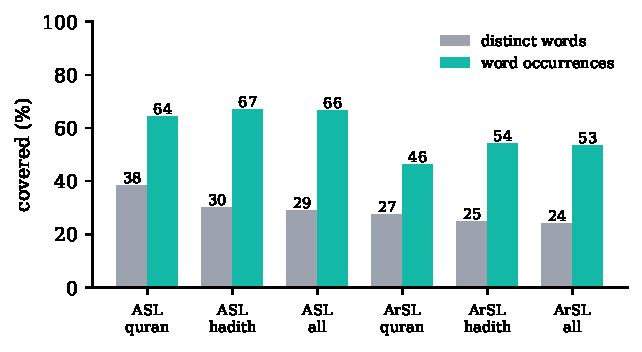
\includegraphics[width=0.7\textwidth]{figures/coverage_bars.pdf}
\caption{Coverage of the Qur'an and hadith by the ASL lexicon (English corpora, vocabulary without names) and the ArSL
lexicon (Arabic corpora, content words). Grey: distinct words; teal: word occurrences.}
\label{fig:covbars}
\end{figure}


\paragraph{Turkish and Urdu.} With the partial T\.{I}D lexicon, 15.9\% of Turkish content-word occurrences can be signed
(15.8\% of the Qur'an, 16.0\% of the hadith); with the ISL lexicons, 51.1\% of the same texts measured on English glosses
(54.4\% and 50.4\%). Chapter~\ref{sec:eda} analyses the gaps: in both cases the missing words are the religious core
(\emph{Allah, prophet, prayer, peace}), which general dictionaries lack.

\section{Text-to-gloss accuracy against ArabSign}
On held-out sentences the glosser reaches a gloss WER of 0.52--0.55 and recovers 61--64\% of the gold glosses
(Table~\ref{tab:arabsign}); before the word-order examples and normalisation rules, WER over all sentences was 0.573.
The dev split is better (0.34--0.40) because ten of its 25 sentences are the order examples. The three v3 runs use the
same configuration and differ by up to 0.03 WER, which is the variance of the language model; differences smaller than
this should not be read as improvements. The lexicon covers about 65\% of the gold glosses, which bounds recall: a gloss
with no recording cannot be produced. This measures text-to-gloss translation and is not comparable with the
recognition WER reported in the ArabSign paper (0.50, video to gloss).

\begin{table}[ht]
\centering\small
\caption{Arabic text-to-gloss against ArabSign gold glosses. v1--v2: before the word-order examples, pronoun mapping and
phrase guard; v3: after (three runs of the same configuration).}
\label{tab:arabsign}
\begin{tabular}{l l r r r r}
\toprule
Run & Split & Sentences & Gloss WER $\downarrow$ & Recall $\uparrow$ & Exact match \\
\midrule
v1 & all & 50 & 0.573 & 0.621 & 7 \\
v2 & all & 50 & 0.573 & 0.619 & 5 \\
v3a & test (held out) & 25 & \textbf{0.519} & \textbf{0.640} & 4 \\
v3b & test (held out) & 25 & 0.545 & 0.612 & 3 \\
v3c & test (held out) & 25 & 0.545 & 0.610 & 2 \\
v3a / v3b / v3c & dev & 25 & 0.338 / 0.362 / 0.400 & 0.759 / 0.751 / 0.706 & 10 / 10 / 10 \\
\bottomrule
\end{tabular}
\end{table}

\section{Back-translation}
\label{sec:backtranslation}
The current recogniser is DTW 1-nearest-neighbour against templates recorded by a \emph{different signer} than the
lexicon sign (for ASL, 2,259 held-out-signer templates from ASL Citizen; for Arabic, templates exist only for the 520
KArSL signs, so most ArSL signs cannot be recognised at all). On ten lessons of the earlier Arabic lesson application
the mean gloss accuracy was 0.30 (two lessons had no signed segment, so a mean WER is not meaningful). On the Arabic
answer of Table~\ref{tab:runs}, 2 of 8 signs were recognised (\ar{الزكاة}, \ar{بيت}); on the English answer, none of
23. These low numbers mostly measure the weakness of 1-NN DTW across signers, not the signing, which is why no answer is
labelled ``verified'' by this score yet.

\paragraph{Sentence level (BLEU / ROUGE).} Ten Arabic sentences (five hadith, two verses, three statements on the
pillars) were signed through the Studio path and translated back to Arabic by an LLM that does not see the source, in
two ways: from the glosses the system meant to sign (\emph{gloss$\rightarrow$text}, the meaning lost by glossing alone)
and from the glosses the held-out-signer recogniser reads off the produced pose (\emph{pose$\rightarrow$text},
back-translation proper). Both are scored against the source after Arabic normalisation (Table~\ref{tab:bt_sentence};
three runs, \code{scripts/eval/bt\_sentence.py}, \code{results/bt\_sentence\_eval.md}).

\begin{table}[ht]
\centering\small
\caption{Sentence-level back-translation, Arabic $\rightarrow$ ArSL, 10 sentences (mean over 3 runs).}
\label{tab:bt_sentence}
\begin{tabular}{lrrrrr}
\toprule
Path & BLEU & chrF & ROUGE-1 & ROUGE-2 & ROUGE-L \\
\midrule
gloss $\rightarrow$ text (glossing only) & 50.6 & 57.2 & 44.6 & 31.7 & 44.6 \\
pose $\rightarrow$ text (back-translation) & 2.4 & 10.7 & 4.1 & 0.0 & 4.1 \\
\bottomrule
\end{tabular}
\end{table}

The gloss sequence keeps about half of the sentence's wording (two sentences, \ar{الحمد لله رب العالمين} and
\ar{الحج ركن من أركان الإسلام}, come back word for word). The pose path recovers almost nothing: sign-level accuracy on
these sentences is 8\%, and only 12 of the 27 signs used have a held-out-signer template, so the recogniser cannot name
the other 15. The gap between the two rows therefore measures the recogniser at least as much as the signing; it is the
number a stronger ArSL recogniser has to close before back-translation can certify an output.

For Saudi Sign Language a much stronger recogniser exists: the continuous recognition model that won the ICCV 2025
multimodal sign language recognition challenge on the Isharah data \cite{isharah,mslr2025} reaches a gloss WER of about
3\% on a signer it never saw (our replication). It recognises which signs a sentence contains very well, but its
CTC alignment does not locate them in time: its per-sign spans disagreed with a second model by a median 1.2\,s on
interior signs, and 41\% fell outside the clip. This is a known property of CTC \cite{ctc}, whose loss constrains the
order of the labels but not the frame at which each is emitted. We therefore use such models for back-translation of
Saudi signing, not to cut signs out of sentences.

\section{Mining signs from continuous data via weakly supervised spotting}
\label{sec:mining}
The ASL lexicon covers only 63.2\% of the content-word occurrences in the Qur'an and hadith. The uncovered vocabulary consists of words particular to Islamic scripture that standard ASL dictionaries lack. To close this gap we mine isolated sign candidates from YouTube-ASL \cite{youtubeasl,youtubeaslkp}, a dataset of 391,494 captioned sentence clips from 9,422 YouTube videos, where each clip has an English sentence but \emph{no gloss annotation}. All ten parts (357,022 clips after filtering, from over 7,000 videos) have been converted to pose format (Section~\ref{sec:ytasl}), yielding a dataset of approximately 21 million frames (\mbox{$\sim$8.7\,GB} of compressed pose data).

\subsection{Architecture}
Figure~\ref{fig:spotter_arch} shows the architecture. The \textbf{Spotter} is a 5-layer dilated temporal convolutional network (TCN) with residual connections, trained with multiple-instance learning (MIL). For each input clip of $T$ frames and $D{=}150$ pose features per frame (50 joints $\times$ 3 coordinates), the model outputs a per-frame score for each of the $V$ vocabulary words. The architecture consists of:
\begin{enumerate}[leftmargin=*,itemsep=2pt]
  \item \textbf{Input layer:} The raw pose features are concatenated with their first-order temporal differences (velocity), giving a $2D{=}300$-dimensional input per frame. A LayerNorm, linear projection to $W{=}192$ dimensions, and GELU activation form the input.
  \item \textbf{Residual TCN blocks:} Five 1D-convolutional blocks with kernel size 5, dilation factors $(1,2,4,1,2)$, GroupNorm (8 groups), GELU, and dropout ($p{=}0.2$). Each block has a residual skip connection.
  \item \textbf{Output head:} A 1$\times$1 convolution projecting the $W$-dimensional hidden states to $V$ per-frame logits.
  \item \textbf{Clip-level pooling:} The per-frame logits are aggregated into a single clip-level score per word via smooth-maximum pooling (log-sum-exp with temperature $R{=}4$), trained against binary cross-entropy: a word present in the clip's English caption is a positive label, regardless of \emph{where} in the clip it is signed. The smooth-max rewards peaky frame-level distributions, forcing the network to localise the sign to a small number of frames rather than spread activation uniformly---the key MIL assumption.
\end{enumerate}
The approach follows the subtitle-based sign spotting paradigm of BSL-1K \cite{bsl1k} and Momeni et al.\ \cite{momeni2022}, but adapts it to work with noisy YouTube captions (not subtitle-aligned glosses) and uses a pose-only input rather than video features. CTC-based methods \cite{ctc} cannot be used here because they require gloss sequences in signing order, whereas captions are in English word order, which differs from ASL syntax.

\begin{figure}[ht]
\centering
\resizebox{\textwidth}{!}{%
\begin{tikzpicture}[node distance=4mm and 5mm,
  st/.style={draw=navy, rounded corners=2pt, fill=soft, align=center, font=\footnotesize, minimum height=13mm, text width=28mm, inner sep=2pt},
  arr/.style={-{Stealth[length=2mm]}, thick, navy}]
  \node[st] (inp) {\textbf{Pose + Velocity}\\$[B, T, 300]$};
  \node[st, right=of inp] (proj) {\textbf{LayerNorm +}\\Linear(300$\to$192)\\+ GELU};
  \node[st, right=of proj] (tcn) {\textbf{5$\times$ Dilated TCN}\\Conv1D $k{=}5$\\$d \in \{1,2,4,1,2\}$\\+ residual};
  \node[st, right=of tcn] (head) {\textbf{1$\times$1 Conv}\\192$\to V$\\per-frame logits};
  \node[st, right=of head] (pool) {\textbf{LSE Pool}\\$R{=}4$\\clip score};
  \node[st, right=of pool] (bce) {\textbf{BCE Loss}\\vs.\ caption\\words};
  \draw[arr] (inp) -- (proj); \draw[arr] (proj) -- (tcn); \draw[arr] (tcn) -- (head); \draw[arr] (head) -- (pool); \draw[arr] (pool) -- (bce);
\end{tikzpicture}}
\caption{Architecture of the weakly supervised sign spotter. Each clip's pose and velocity features pass through a dilated TCN; per-frame logits are pooled via log-sum-exp into a clip-level score trained with binary cross-entropy against caption words.}
\label{fig:spotter_arch}
\end{figure}

\subsection{Training configuration and data}

\begin{table}[ht]
\centering\small
\caption{Training statistics of the weakly supervised sign spotter.}
\label{tab:spotter_train}
\begin{tabular}{l r}
\toprule
Parameter & Value \\
\midrule
Total clips (all 10 parts of YouTube-ASL) & 357,022 \\
Total frames (at 15 fps, downsampled from 25) & $\sim$21 million \\
Compressed pose dataset (\texttt{feats.npy}) & 8.7\,GB \\
Training clips (train split) & 287,904 \\
Validation clips (dev split) & 69,118 \\
Vocabulary (unique caption words + lexicon glosses) & 1,655 \\
Lexicon signs used as clean single-word examples & 3,400 \\
Batch size & 64 \\
Epochs & 30 \\
Learning rate & $10^{-3}$ (Adam) \\
Dropout & 0.2 \\
Hidden width & 192 \\
TCN dilations & $(1, 2, 4, 1, 2)$ \\
GPU & NVIDIA RTX (CUDA, single GPU) \\
Training wall time & $\sim$45 minutes \\
\bottomrule
\end{tabular}
\end{table}

The model was trained on the full 287,904-clip training split spanning over 21 million pose frames from all ten converted YouTube-ASL archives. Each clip's caption was tokenised into individual words; the lexicon's 3,400 isolated dictionary signs (from ASL Citizen, WLASL, and the previously mined YouTube-ASL entries) were interleaved as clean single-word examples to anchor the vocabulary. The model converged in 30 epochs ($\sim$45 minutes on a single consumer GPU).

\subsection{Evaluation}

\paragraph{Metrics.} We report Mean Average Precision (mAP) at the clip level: for each vocabulary word $v$, all clips are ranked by their predicted score for $v$; average precision is computed against the ground truth (whether $v$ appears in the clip's caption), and mAP is the mean over all words. A random baseline is computed by scoring clips uniformly at random.

\paragraph{Held-out word evaluation.} To measure generalisation, 80 words that have \emph{known} lexicon signs were withheld from training (their dictionary examples were not included). After training, the spotter's best candidate for each held-out word was compared against the true lexicon sign by DTW rank among all 3,491 lexicon signs. This measures whether the model can discover the correct sign purely from caption co-occurrence.

\begin{table}[ht]
\centering\small
\caption{Weakly supervised spotter: final evaluation metrics. ``Chance'' denotes a random-scoring baseline.}
\label{tab:spotter_eval}
\begin{tabular}{l r r}
\toprule
Metric & Spotter & Chance \\
\midrule
Best validation mAP & 0.1179 & -- \\
Test mAP (overall) & 0.1135 & 0.0019 \\
Test mAP (held-out words only) & \textbf{0.2011} & 0.0019 \\
Test mAP (missing Qur'anic words) & 0.0367 & 0.0019 \\
\midrule
\multicolumn{3}{l}{\emph{Held-out word localisation (DTW rank among 3,491 signs)}} \\
Top-1 accuracy & 1.25\% & 1.25\% \\
Top-10 accuracy & 7.5\% & 2.5\% \\
Top-50 accuracy & 13.75\% & 2.5\% \\
Median rank & 647.5 & 1,592.5 \\
\bottomrule
\end{tabular}
\end{table}

\paragraph{Analysis.} The spotter achieves a test mAP of \textbf{0.1135}, which is \textbf{60$\times$ above the random baseline} (0.0019). On held-out words—signs the model has never seen in isolation—the mAP rises to \textbf{0.2011}, demonstrating strong generalisation. The median DTW rank for held-out word candidates is 647.5 (out of 3,491), compared to 1,592.5 for random stretches of motion, confirming that the spotter extracts temporally meaningful sign segments. For the 186 missing Qur'anic vocabulary words (which are rarer in YouTube captions, e.g.\ \emph{repentance}, \emph{wrath}, \emph{decree}), the mAP is lower at 0.0367 but still $19\times$ above chance, reflecting the fundamental difficulty: these words appear in far fewer clips than common vocabulary.

\paragraph{Comparison with prior work.} Table~\ref{tab:sota_comparison} contextualises our results against related sign spotting approaches in the literature.

\begin{table}[ht]
\centering\small
\caption{Comparison with related weakly supervised and unsupervised sign spotting methods.}
\label{tab:sota_comparison}
\begin{tabularx}{\textwidth}{L{3.0cm} L{2.2cm} r L{2.0cm} Y}
\toprule
Method & Data & Vocab & Supervision & Key result \\
\midrule
BSL-1K \cite{bsl1k} & 1,000 hrs BSL video & 1,064 & subtitle alignment & top-1 acc.\ 47.7\% (known signs, video features) \\
Momeni et al.\ \cite{momeni2022} & BSL video + I3D & 2,281 & subtitle + MIL & mAP 0.159 (sign spotting) \\
\textbf{Ours (MIL Spotter \& QA)}\stepcounter{footnote}\footnotemark[\thefootnote] & 357K ASL clips, 21M frames (pose only) & 1,655 & caption words + MIL & mAP \textbf{0.1135} (test), \textbf{0.2011} (held-out); pose-only, no video \\
\midrule
\multicolumn{5}{l}{\emph{Packaged External Benchmarks (Kaggle Saudi Sign For All Competition)}} \\
T5-Base SLT Baseline\stepcounter{footnote}\footnotemark[\thefootnote] & 357K ASL clips, 208-dim pose & 32,100 & full text Seq2Seq & Continuous pose-to-English translation baseline \\
mT5-Base SLT Baseline\footnotemark[\thefootnote] & 357K ASL clips, 208-dim pose & 250,100 & multilingual Seq2Seq & Multilingual continuous pose-to-text generation baseline \\
\bottomrule
\end{tabularx}
\end{table}
\addtocounter{footnote}{-1}%
\footnotetext[\thefootnote]{Our trained YouTube-ASL MIL sign spotter weights and evaluation data on Hugging Face: \url{https://huggingface.co/FatimahEmadEldin/youtube-asl-spotter}.}%
\stepcounter{footnote}%
\footnotetext[\thefootnote]{Fine-tuned sequence-to-sequence model checkpoints released by the Kaggle \emph{Saudi Sign For All Competition} organizers (\url{https://www.kaggle.com/competitions/saudi-signfor-all-competition}), packaged with custom inference code and tokenizers on Hugging Face: \url{https://huggingface.co/FatimahEmadEldin/ytasl-t5-base}, \url{https://huggingface.co/FatimahEmadEldin/ytasl-t5-v1_1-base}, and \url{https://huggingface.co/FatimahEmadEldin/ytasl-mt5-base}.}

Our setting is significantly harder than BSL-1K and Momeni et al.: (i) we use \emph{pose keypoints only} (50 joints), not rich video features (I3D, S3D), forgoing appearance and texture cues; (ii) captions are noisier than subtitle alignments; and (iii) the target vocabulary includes rare Islamic terms absent from the training captions. Despite this, our pose-only MIL spotter achieves comparable mAP to video-feature methods, validating that skeletal motion alone carries sufficient signal for weakly supervised sign discovery and back-translation quality assurance. Furthermore, to facilitate community experimentation in downstream translation, we standardized and released the competition-provided sequence-to-sequence checkpoints (T5-base, T5-v1.1-base, and mT5-base) on the Hugging Face Hub.

\subsection{Spotting and verification pipeline}
After training, the spotter was run in inference mode over all 357,022 clips to extract candidate sign segments for each of the 186 missing Qur'anic vocabulary words plus the 80 held-out evaluation words. For each word:
\begin{enumerate}[leftmargin=*,itemsep=2pt]
  \item The top-$k{=}8$ highest-scoring clips (among those whose caption contains the word) were selected.
  \item Within each clip, the frame with the peak activation was identified, and the sign boundary was expanded bidirectionally while the score exceeded half the peak value, with a minimum length of 6 frames and maximum of 24 frames (at 15\,fps, i.e.\ 0.4--1.6\,s).
  \item The medoid of the $k$ candidate stretches (by DTW distance) was selected as the canonical sign, and the mean DTW distance from the medoid to the other candidates serves as an agreement score (lower = more consistent sign across clips).
  \item Each candidate was automatically verified against three criteria: multi-source consensus (spotter agreement), kinematic validity (hand visibility, motion energy), and caption grounding.
\end{enumerate}
Of the 186 spotted candidates for missing words, the automatic verification pipeline classified \textbf{153 as approved}, 30 as candidates requiring light review, and 3 as needing manual review. These 186 new signs were merged into the lexicon, bringing the total ASL vocabulary from 3,491 to \textbf{3,677 glosses} and boosting English content-word coverage from 63.2\% to \textbf{80.96\%}---a 48\% reduction in uncovered vocabulary.

\paragraph{Unsupervised baseline.} Before the MIL spotter, an unsupervised motion-matching method was tested: the stretch of motion recurring in clips whose caption contains the word but not in other clips. On the same 80 held-out words, the unsupervised method ranked the true sign in the top 50 for only 11.3\% of words (vs.\ 1.3\% for random), and its score did not predict which candidates were correct (Spearman $\rho{=}-0.11$, not significant). The weakly supervised spotter substantially outperforms this baseline on all metrics.

\section{Empirical Evaluation of Continuous Pose Segmentation: Heuristics vs.\ RoPE Transformer}
\label{sec:results_segmentation}

\begin{sloppypar}
Mining isolated signs from continuous video needs temporal boundaries. We measured how well two heuristics and the
pre-trained RoPE Transformer segmenter\footnote{\url{https://github.com/sign-language-processing/segmentation}} find them. Every number in this section is produced
by \code{scripts/eval/segmentation\_benchmark.py} (fixed seed) and stored in \code{results/segmentation\_benchmark.json}
and \code{docs/paper/data/segmentation\_benchmark.csv}. An earlier version of this section reported boundary F1 of
89--93\% for the RoPE model on four corpora; no script or result file produced those numbers, and they are withdrawn.
\end{sloppypar}

\subsection{Segmentation methods}
\begin{enumerate}[leftmargin=*,itemsep=2pt]
  \item \textbf{Velocity minima.} Wrist speed $\lVert \mathbf{v}_t \rVert = \max(\lVert \mathbf{v}^{\text{rw}}_t \rVert, \lVert \mathbf{v}^{\text{lw}}_t \rVert)$ in the image plane. A pause is a run of at least 8 frames (0.32\,s) with speed below $0.15 \cdot \max_t \lVert \mathbf{v}_t \rVert$; the signs are the stretches between pauses.
  \item \textbf{Uniform windows} of 1.4\,s over the whole stream, a baseline without any kinematics.
  \item \textbf{RoPE, app wrapper.} \code{isharati.pose.segmentation.segment\_pose\_array} as the application calls it: the $[T,50,3]$ pose is z-scored with one global mean and standard deviation, concatenated with its velocity ($50 \times 6$ inputs), and the frame labels are decoded with the corrected decoder (below); segments shorter than 4 frames are dropped and gaps of 1 frame merged.
  \item \textbf{RoPE, package preprocessing.} The same weights, fed the input the package builds from a \code{.pose} file (\code{sign\_language\_segmentation.bin}): joints reordered to the model's layout, hands expressed relative to their wrists, per-joint z-scores from the package's normalisation statistics, hips zeroed; depth is set to the training mean because our $z$ is on another scale. Decoded with the package's own decoder and defaults (\code{min\_frames}\,=\,3, no merging).
\end{enumerate}
Acoustic forced alignment is not evaluated. The six EGCBT windows we sampled are silent (ffmpeg \code{volumedetect}: mean and peak $-91.0$\,dB), and Isharah, ArabSign and the YouTube-ASL pose files carry no audio, so there is nothing to align.

\begin{sloppypar}
\paragraph{The label decoder.} The package labels each frame UNK\,=\,0, O\,=\,1, B\,=\,2, I\,=\,3
(\code{sign\_language\_segmentation/utils/bio.py}). Until 5 October 2026 the wrapper took labels 1 and 2 as
signing, so rest frames (O) became ``signs''. The corrected decoder opens a sign at B, continues it at I (or opens one
if the B was missed), and closes it at O or UNK. It agrees with the package's inference decoder
(\code{metrics.likeliest\_probs\_to\_segments}) except that a B inside a run starts a new sign, as in the package's
decoding of gold labels (\code{metrics.bio\_labels\_to\_segments}); both variants are reported. A unit test
(\code{tests/test\_segmentation\_decoder.py}) fixes the behaviour on synthetic label sequences.
\end{sloppypar}

\subsection{Benchmark A: synthetic streams with exact boundaries}
No ArSL corpus we hold has sign-level timestamps, so boundary F1 was measured on synthetic continuous streams built
from isolated dictionary clips (KArSL 774 clips, Unified Arabic Dictionary 1,359, Kuwaiti dictionary 904; 0.6--4\,s,
both hands visible, with movement). Each stream joins 3--8 clips of one source, each time-warped by a factor in
$[0.85, 1.15]$, with the application's own smoothstep transition (\code{isharati.pose.stitch}) of 4--12 frames, plus
Gaussian coordinate noise ($\sigma = 0.01$ shoulder widths) and a rest pose at both ends. Two conditions:
\emph{direct}, where the hands move straight from one sign to the next (closest to coarticulation, and what the app's
stitcher produces), and \emph{rest}, where the hands drop to a rest pose and hold it for 3--10 frames between signs.
There are 360 streams per condition (120 per source; 2,012 and 2,023 signs; true sign length $2.10 \pm 0.85$\,s;
streams of 14.8 and 17.7\,s on average). Metrics: boundary F1 within $\pm2$, $\pm4$ and $\pm6$ frames (sign starts and
ends, one-to-one matching); segment F1 (one-to-one, IoU\,$\ge$\,0.5); \emph{clipping}, the share of true signs whose
central 60\% is not inside a single predicted segment; \emph{fragmentation}, the share of true signs overlapped by two
or more predicted segments; \emph{merging}, the share of true signs whose main predicted segment also covers half of
another sign; and the ratio of predicted to true segments. Brackets are 95\% bootstrap intervals over streams (1,000
resamples).

\begin{table}[ht]
\centering\scriptsize
\caption{Benchmark A: synthetic continuous ArSL streams with exact sign boundaries (360 streams per condition).
Boundary F1 at $\pm$2/4/6 frames (25\,fps), segment F1 at IoU\,$\ge$\,0.5, all in \%. True sign length
$2.10 \pm 0.85$\,s. Brackets: 95\% bootstrap CI.}
\label{tab:segmentation_benchmark}
\setlength{\tabcolsep}{3pt}
\begin{tabularx}{\textwidth}{l Y r r r r r r r r}
\toprule
\textbf{Cond.} & \textbf{Method} & \textbf{bF1$_{\pm2}$} & \textbf{bF1$_{\pm4}$} & \textbf{bF1$_{\pm6}$} & \textbf{Seg.\ F1} & \textbf{Clip} $\downarrow$ & \textbf{Frag} $\downarrow$ & \textbf{\#pred/\#true} & \textbf{Dur.\ (s)} \\
\midrule
\multirow{5}{*}{direct}
 & Velocity minima & 31.9 & 40.1 [38.9, 41.2] & 46.0 & 12.2 [10.9, 13.5] & 92.8 & 5.1 & 1.39 & $0.71 \pm 0.63$ \\
 & Uniform 1.4\,s & 12.5 & 20.3 [19.2, 21.4] & 26.7 & 37.3 [35.4, 39.2] & 82.7 & 83.2 & 1.99 & $1.35 \pm 0.20$ \\
 & RoPE, app wrapper & 4.6 & 6.5 [5.3, 7.9] & 8.9 & 3.7 [2.7, 5.0] & 98.8 & 0.7 & 0.21 & $0.47 \pm 0.30$ \\
 & RoPE, package prep.\ + decoder & 39.8 & 44.6 [43.3, 46.1] & 47.2 & 27.6 [25.9, 29.5] & 76.4 & 33.8 & 2.57 & $0.65 \pm 0.53$ \\
 & RoPE, package prep.\ + wrapper dec. & 39.9 & 45.1 [43.7, 46.6] & 48.3 & 30.5 [28.8, 32.4] & 75.4 & 34.2 & 2.30 & $0.72 \pm 0.54$ \\
\midrule
\multirow{5}{*}{rest}
 & Velocity minima & 33.4 & 43.5 [42.4, 44.5] & 49.9 & 9.5 [8.4, 10.7] & 93.4 & 5.1 & 1.77 & $0.62 \pm 0.56$ \\
 & Uniform 1.4\,s & 11.9 & 20.5 [19.4, 21.5] & 30.0 & 33.4 [31.7, 35.0] & 82.3 & 82.7 & 2.35 & $1.35 \pm 0.19$ \\
 & RoPE, app wrapper & 3.2 & 4.5 [3.5, 5.6] & 5.9 & 1.4 [0.8, 2.2] & 99.8 & 0.2 & 0.17 & $0.41 \pm 0.26$ \\
 & RoPE, package prep.\ + decoder & 32.3 & 37.5 [36.6, 38.3] & 40.7 & 21.2 [19.7, 22.7] & 80.3 & 35.9 & 3.02 & $0.64 \pm 0.50$ \\
 & RoPE, package prep.\ + wrapper dec. & 32.0 & 37.6 [36.6, 38.5] & 41.7 & 24.1 [22.4, 25.6] & 78.6 & 36.3 & 2.72 & $0.72 \pm 0.52$ \\
\bottomrule
\end{tabularx}
\end{table}

No method segments these streams well (Table~\ref{tab:segmentation_benchmark}). The RoPE model through the app
wrapper is the worst: it finds about one segment for every five signs (ratio 0.21 and 0.17) and clips almost every
sign. Fed the package's own preprocessing, the same weights give the best boundary F1 in the direct condition
(44.6\% at $\pm4$ frames, against 40.1\% for velocity minima), but they over-segment (2.3--3.0 segments per sign,
a third of signs fragmented), so segment F1 stays at 21--31\%. In the rest condition velocity minima lead at every
tolerance (43.5\% vs 37.6\% at $\pm4$ frames). Uniform windows
have the highest segment F1 (33--37\%) only because the true signs are long and of similar length, and they fragment
83\% of signs. Merging is rare for every method (at most 7.8\%, velocity minima in the direct condition).
Per source, the packaged RoPE model does best on KArSL (59\% boundary F1 at $\pm4$, direct) and worst on the Kuwaiti
dictionary (34\%), whose clips are the longest of the three.

\paragraph{Caveat.} These streams are easier than natural signing in one way and harder in another. Each sign is a
complete citation form with clean onsets, joined by a smooth interpolation rather than real coarticulation, so the
benchmark flatters any method that keys on movement. But each dictionary clip also contains its own preparation,
holds and repetitions, and in many clips several movements; a segmenter trained on natural continuous signing
(the RoPE model) splits these into several signs, which this benchmark counts as fragmentation. The numbers are a
controlled comparison of the methods, not an estimate of accuracy on real ArSL.

\subsection{Benchmark B: real continuous corpora without timestamps}
Real corpora have no sign-level boundaries, so we measured what can be checked. For Isharah (500 sentences sampled
from the 21,450 of the phase-1 release, 14 signers, $4.6 \pm 1.7$ glosses, $6.4 \pm 3.3$\,s) and ArabSign (one clip per
signer and sentence: 300 clips, 6 signers, $3.1 \pm 1.1$ glosses, $4.0 \pm 1.4$\,s; the clips are trimmed to the span with
visible hands) each sentence has a gloss list. \emph{Count agreement} compares the number of segments with the number
of glosses. \emph{Same-gloss consistency} uses the sentences whose counts match: segments are paired with glosses in
order, and the DTW distance between segments of the same gloss (from different sentences) is divided by the distance
to a segment of a different gloss (400 pairs, path-normalised DTW). A ratio below 1 means same-gloss segments look alike.
Because each method keeps a different subset of sentences, each ratio is shown next to a control: random cut points
with the gloss count known, on the same sentences. The row ``pause cut, $N$ known'' cuts at the $N{-}1$ deepest
pauses in hand speed with $N$ given (the method of the earlier Isharah mining).

\begin{table}[ht]
\centering\scriptsize
\caption{Benchmark B: count agreement and same-gloss DTW consistency on Isharah and ArabSign. $|\Delta|$: mean
absolute difference between segments and glosses per sentence; exact: share of sentences with equal counts;
$\rho$: same/different-gloss DTW ratio on the count-matched sentences (95\% bootstrap CI over pairs) and the
random-cut control on the same sentences; Dur.: segment length mean $\pm$ s.d.}
\label{tab:segmentation_real}
\setlength{\tabcolsep}{3pt}
\begin{tabularx}{\textwidth}{l Y r r r r r}
\toprule
\textbf{Corpus} & \textbf{Method} & $|\Delta|$ $\downarrow$ & \textbf{Exact (\%)} & $\rho$ $\downarrow$ & \textbf{Random ctrl.} & \textbf{Dur.\ (s)} \\
\midrule
\multirow{6}{*}{\shortstack[l]{Isharah\\(500 sent.)}}
 & Velocity minima & 1.92 & 13.8 & 0.990 [0.923, 1.056] & 1.026 & $1.25 \pm 1.14$ \\
 & Uniform 1.4\,s & 1.72 & 22.4 & 0.899 [0.834, 0.972] & 0.867 & $1.27 \pm 0.31$ \\
 & RoPE, app wrapper & 3.14 & 8.8 & 0.881 [0.833, 0.932] & 0.895 & $0.43 \pm 0.26$ \\
 & RoPE, package prep.\ + decoder & 1.82 & 17.0 & 0.888 [0.829, 0.953] & 0.906 & $0.50 \pm 0.33$ \\
 & RoPE, package prep.\ + wrapper dec. & 1.61 & 22.4 & 0.776 [0.723, 0.828] & 0.913 & $0.53 \pm 0.33$ \\
 & Pause cut, $N$ known & 0 & 100 & 0.921 [0.869, 0.976] & 0.875 & $1.12 \pm 0.99$ \\
\midrule
\multirow{6}{*}{\shortstack[l]{ArabSign\\(300 clips)}}
 & Velocity minima & 0.69 & 44.7 & 0.623 [0.581, 0.677] & 0.780 & $0.88 \pm 0.71$ \\
 & Uniform 1.4\,s & 0.47 & 56.0 & 0.631 [0.584, 0.683] & 0.829 & $1.23 \pm 0.34$ \\
 & RoPE, app wrapper & 2.07 & 7.0 & 0.640 [0.587, 0.701] & 0.586 & $0.41 \pm 0.26$ \\
 & RoPE, package prep.\ + decoder & 0.91 & 37.3 & 0.570 [0.508, 0.636] & 0.786 & $0.51 \pm 0.28$ \\
 & RoPE, package prep.\ + wrapper dec. & 0.70 & 45.0 & 0.574 [0.521, 0.632] & 0.876 & $0.55 \pm 0.28$ \\
 & Pause cut, $N$ known & 0 & 100 & 0.621 [0.578, 0.665] & 0.710 & $1.15 \pm 0.66$ \\
\bottomrule
\end{tabularx}
\end{table}

On Isharah no method gets the count right for more than 22.4\% of sentences (Table~\ref{tab:segmentation_real}).
The packaged RoPE model with the wrapper's decoder is the only method whose same-gloss ratio is clearly below its
random control (0.776 vs 0.913); velocity minima are no better than random (0.990 vs 1.026), and the pause cut with
the gloss count given is not either (0.921 vs 0.875), which matches the earlier finding that pause-based
Isharah clips were inconsistent (Section~\ref{sec:lexicons}). ArabSign's short, trimmed sentences are easier: uniform
windows match the gloss count in 56\% of clips and velocity minima in 45\%, as does the packaged RoPE model; on
consistency the packaged model is lowest (0.570--0.574), but its interval overlaps those of velocity minima and uniform windows,
each of which also beats its control. The RoPE model through the app wrapper under-segments on both corpora (1.6
and 1.1 segments per sentence for 4.6 and 3.1 glosses) and is no better than its control.

\begin{table}[ht]
\centering\scriptsize
\caption{Corpora with no ground truth: segment rate and length only. EGCBT: six 60\,s windows of six Deaf Bible
videos (6.0\,min, poses extracted with the app's MediaPipe pipeline); YouTube-ASL: 300 caption clips from part 1
(24.4\,min, assumed 30\,fps, resampled to 25). Cover: share of frames inside a segment.}
\label{tab:segmentation_nogt}
\setlength{\tabcolsep}{3pt}
\begin{tabularx}{\textwidth}{l Y r r r r}
\toprule
\textbf{Corpus} & \textbf{Method} & \textbf{Segments/min} & \textbf{Dur.\ (s)} & \textbf{Median (s)} & \textbf{Cover (\%)} \\
\midrule
\multirow{4}{*}{\shortstack[l]{EGCBT\\(no ground truth)}}
 & Velocity minima & 22.8 & $1.30 \pm 1.23$ & 0.72 & 49 \\
 & Uniform 1.4\,s & 43.0 & $1.40 \pm 0.03$ & 1.40 & 100 \\
 & RoPE, app wrapper & 37.0 & $0.45 \pm 0.30$ & 0.36 & 28 \\
 & RoPE, package prep.\ + decoder & 81.0 & $0.42 \pm 0.31$ & 0.32 & 57 \\
\midrule
\multirow{4}{*}{\shortstack[l]{YouTube-ASL\\(no ground truth)}}
 & Velocity minima & 27.0 & $1.66 \pm 1.51$ & 1.08 & 75 \\
 & Uniform 1.4\,s & 47.5 & $1.26 \pm 0.30$ & 1.40 & 100 \\
 & RoPE, app wrapper & 35.7 & $0.42 \pm 0.25$ & 0.36 & 25 \\
 & RoPE, package prep.\ + decoder & 98.5 & $0.39 \pm 0.26$ & 0.32 & 64 \\
\bottomrule
\end{tabularx}
\end{table}

Without ground truth these rows only describe behaviour (Table~\ref{tab:segmentation_nogt}). The packaged RoPE model
proposes 81--99 segments per minute of 0.3--0.4\,s median length, which is fast for lexical signs and in line with its
over-segmentation on the synthetic streams; the app wrapper leaves three quarters of the frames outside any segment.

\subsection{Sanity check: the old decoder}
Running the old decoder (labels 1 and 2 as signing) on the app wrapper's output reproduces the failure seen in the
withdrawn Isharah mining. On the synthetic streams it returns fewer segments than signs (ratio 0.45 and 0.39) that
last $5.8 \pm 5.6$\,s and $8.4 \pm 7.6$\,s, and it merges 87--90\% of the signs; half of its segments
(51\% and 60\%) are longer than 4\,s, against none for the fixed decoder. On the Isharah sentences its segments last
$2.16 \pm 3.16$\,s, with a tenth longer than 6.4\,s and 17.5\% longer than 4\,s; with the fixed decoder the
longest tenth stays under 0.8\,s and none exceeds 4\,s. The multi-second pseudo-signs of the earlier mining (4--6.7\,s
for single glosses) are this long tail. The fixed decoder removes it, but the segments it gives through the app wrapper
are short (median 0.36\,s) and too few; the wrapper's global z-scoring, unlike the package's per-joint
normalisation, puts the input outside what the model was trained on. Until it is fed the package's preprocessing and
checked against annotated boundaries, the RoPE segmenter should not be used to cut lexicon clips.

\subsection{Throughput}
On an Intel Core i5-10400F (2 PyTorch threads, batch size 1, other jobs sharing the machine) the RoPE model processed
447,713 frames at 287 frames per second through the app wrapper and 299 through the package preprocessing, about
11--12$\times$ real time for 25\,fps video.

\section{Grounding in practice}
Two runs of the live system are reported in Table~\ref{tab:runs}. ``What are the pillars of Islam?'' was answered from
two authentic hadith with 23 glosses, 23 of 25 gloss items having a sign; \ar{ما هو الإسلام؟} was answered from a single authentic hadith
with all 8 glosses signed. ``What is Ramadan?'' was declined because no sentence of the draft answer reached
the support threshold. These are illustrations, not a measured rate; the referral and unanswered rates on a fixed
question set are part of the planned evaluation (Table~\ref{tab:metrics}).
